\documentclass[
    oneside,         % oneside/twoside : Einseitiger oder zweiseitiger Druck?
    10pt,            % Bezug: 12-Punkt Schriftgre
    DIV15,           % Randaufteilung, siehe Dokumentation "KOMA"-Script
    BCOR17mm,        % Bindekorrektur: Innen 17mm Platz lassen. Copyshop-getestet.
    headsepline,     % Unter Kopfzeile Trennlinie (aus: headnosepline)
    footsepline,     % ber Fuzeile Trennlinie (aus: footnosepline)
    openright,       % Neue Kapitel im zweiseitigen Druck rechts beginnen lassen
    a4paper,         % Seitenformat A4
    abstracton,      % Abstract einbinden
    english,
    listof=totoc,version=first,      % Div. Verzeichnisse ins Inhaltsverzeichnis aufnehmen
    bibliography=totoc,version=first,        % Literaturverzeichnis ins Inhaltsverzeichnis aufnehmen
    titlepage,       % Titelseite aktivieren
    headinclude,     % Seiten-Head in die Satzspiegelberechnung mit einbeziehen
    footexclude,     % Seiten-Foot nicht in die Satzspiegelberechnung mit einbeziehen
    numbers=noenddot,version=first % Gliederungsnummern ohne abschlieenden Punkt darstellen
] {scrreprt}       % Dokumentenstil: "Report" aus dem KOMA-Skript-Paket

\usepackage[active]{srcltx}
%\usepackage[activate=normal]{pdfcprot\documentclass[options]{class}} % Optischer Randausgleich -> pdflatex!
\usepackage{ifthen}
\usepackage[english,ngerman]{babel}
%\usepackage[english]{babel}
%\usepackage{ngerman}
%\usepackage[fixlanguage]{babelbib}
%\setbiblanguage{english}
\usepackage[latin1]{inputenc}
\usepackage[T1]{fontenc}
\usepackage[T1]{url}
\usepackage{ae}
\usepackage[final]{graphicx}
\usepackage[automark]{scrlayer-scrpage}
\usepackage{setspace}
\usepackage{floatflt} 
\usepackage{rotating} 
\usepackage{wrapfig}
%\usepackage{subfig}
\usepackage{graphicx}
%\usepackage[first,light]{draftcopy} % Fr Probedruck
\usepackage[plainpages=false,pdfpagelabels,hypertexnames=false]{hyperref}
\usepackage{pdfpages}   %include pdf files
\usepackage{listings} %include sourcecode
\usepackage{color}
\definecolor{commentgreen}{rgb}{0,0.5,0}
\usepackage{multirow}
\usepackage{verbatim}
\usepackage{amsmath}
\usepackage{amssymb}
\usepackage{amsfonts}
\usepackage{enumitem}
\usepackage{setspace}
\usepackage{array}
\usepackage{nomencl}
% \usepackage[table]{xcolor}
\usepackage{longtable}
\usepackage{url}
\usepackage{subcaption}
\usepackage{longtable}
%\usepackage{paralist}
\usepackage{tipa}
\usepackage{csquotes}
%\usepackage{textcomp}  %mit \textcent geht Cent-Symbol


% Tiefe der Kapitelnummerierung beeinflussen
\setcounter{secnumdepth}{3} % Tiefe der Nummerierung
\setcounter{tocdepth}{3}    % Tiefe des Inhaltsverzeichnisses

% Hier in die zweite geschweifte Klammer jeweils
% die persnlichen Daten eintragen:
%\newcommand{\artderausarbeitung}{PhD Thesis}
\newcommand{\artderausarbeitung}{}
%\newcommand{\namedesautors}{Anna Marie Kruspe}
\newcommand{\namedesautors}{}
\newcommand{\inventarisierungsnummer}{}

\newcommand{\markup}[1]{\textbf{#1}}

% Seitenlayout festlegen. Hier nichts ndern!
\pagestyle{scrplain}
\ihead[]{\headmark}
\ohead[]{\pagemark}
\chead[]{}
\ifoot[]{\scriptsize \inventarisierungsnummer}
\ofoot[]{\scriptsize \artderausarbeitung\ \namedesautors}
\cfoot[]{}
\renewcommand{\titlepagestyle}{scrheadings}
\renewcommand{\partpagestyle}{scrheadings}
\renewcommand{\chapterpagestyle}{scrheadings}
\renewcommand{\indexpagestyle}{scrheadings}

% Abschnittsweise Nummerierung anstatt fortlaufend. Hier nichts ndern!
\makeatletter
\@addtoreset{equation}{chapter}
\@addtoreset{figure}{chapter}
\@addtoreset{table}{chapter}
\renewcommand\theequation{\thechapter.\@arabic\c@equation}
\renewcommand\thefigure{\thechapter.\@arabic\c@figure}
\renewcommand\thetable{\thechapter.\@arabic\c@table}\makeatother

% Quelltextrahmen, klein. Hier nichts ndern!
\newsavebox{\inhaltkl}
\def\rahmenkl{\sbox{\inhaltkl}\bgroup\small\renewcommand{\baselinestretch}{1}\vbox\bgroup\hsize\textwidth}
\def\endrahmenkl{\par\vskip-\lastskip\egroup\egroup\fboxsep3mm%
\framebox[\textwidth][l]{\usebox{\inhaltkl}}}

% Quelltextrahmen, normale Groesse. Hier nichts ndern!
\newsavebox{\inhalt}
\def\rahmen{\sbox{\inhalt}\bgroup\renewcommand{\baselinestretch}{1}\vbox\bgroup\hsize\textwidth}
\def\endrahmen{\par\vskip-\lastskip\egroup\egroup\fboxsep3mm%
\framebox[\textwidth][l]{\usebox{\inhalt}}}


% Sonstige Befehlsdefinitionen hier ablegen.
\newcommand{\entspricht}{\stackrel{\wedge}{=}}
\definecolor{light-gray}{gray}{0.95}
\addto\captionsenglish{\renewcommand{\contentsname}{Table of Contents}}
%\makenomenclature
\makeglossary
\DeclareMathOperator*{\argmin}{argmin}
\DeclareMathOperator*{\argmax}{argmax}

\bibliographystyle{IEEEbib}

\begin{document}

    \onehalfspacing
    \clubpenalty=10000
    \widowpenalty=10000
    \selectlanguage{english}
    % \input{chapter/TitlePage.tex}
    % Inhaltsverzeichnis
    \cleardoublepage % Seitenumbruch erzwingen vor nderung des Nummerierungsstils
    \footnotesize
    %\begin{otherlanguage}[english]
    \pagenumbering{roman} % Nummerierung der Seiten ab hier: i, ii, iii, iv...
    \pagestyle{scrheadings} % Ab hier mit Kopf- und Fusszeile

    \normalsize
    % \input{chapter/Abstract.tex}
    % \input{chapter/Acknowledgements.tex}
    \footnotesize
    \tableofcontents

    % Inhaltsverzeichnis
    \cleardoublepage % Seitenumbruch erzwingen vor nderung des Nummerierungsstils
    \normalsize
    \pagenumbering{arabic}
    % !TEX root = ../main.tex

\chapter{Introduction} \label{chap:introduction}
    \section{Motivation} \label{sec:intro_motivation}
        Human action and gesture recognition aims at recognizing an action from a given video clip. This is an attractive research topic, which has been extensively studied over the years due to its broad range of applications from video surveillance to human machine interaction \cite{herath2017going, zhang2019comprehensive}.
        %While action and gesture recognition in constrained simple backgrounds scene taken from common views seems to be a well solved problem, recognizing actions from real-world complex scenes has to face new challenges.
        Within this scope, a very important demand is independence to viewpoint. However, different viewpoints result in various human pose, background, camera motions, lighting conditions and occlusions. Consequently, recognition performance could be dramatically degraded under viewpoint changes.

        To overcome this problem, a number of methods have been proposed. View independence recognition such as \cite{gavrila19963, lv2007single, weinland2007action} \cite{weinland2011survey} generally require a careful multi-view camera setting for robust joint estimation. View invariance approach \cite{junejo2008cross, li2012cross} is usually limited by inherent structure of view-invariant features. Recently, knowledge transfer technique is widely deployed for cross-view action recognition, for instance bipartite graph that bridge the semantic gap across view dependent vocabularies \cite{liu2011cross}, AND-OR graph (MST-AOG) for cross-view action recognition \cite{wang2014cross}. To increase discriminant and informative features, view private features and shared features are both incorporated in such frameworks to learn the common latent space \cite{kong2017deeply, liu2018hierarchically}. 
        While existing works for human action and gesture recognition from common viewpoints explored different deep learning techniques and achieved impressive accuracy. In most of aforementioned multi-view action recognition techniques, the features extracted from each view are usually hand-crafted features (i.e improved dense trajectories) \cite{rahmani2017learning, liu2018hierarchically,kong2017deeply}. Deep learning techniques, if used, handle knowledge transfer among viewpoints. Deployment of deep features in such frameworks for cross-view scenario is under active investigation.
        %To overcome this problem, a number of methods have been proposed. View independence recognition has been surveyed in \cite{weinland2011survey}. View normalization 2D/3D attempts to estimate view transformation between model and observation \cite{gavrila19963, lv2007single, weinland2007action}. These approaches generally require a careful multi-view camera setting for robust joint estimation. View invariance approach searched for features and matching functions that are independent with view changes \cite{junejo2008cross, li2012cross}. The performance of this approach is limited by inherent structure of view-invariant features. Recently, knowledge transfer technique is widely deployed for cross-view action recognition. Liu et al. utilized a bipartite graph to build bilingual words that bridge the semantic gap across view dependent vocabularies \cite{liu2011cross}. Wang et al. introduced a multi-view spatio-temporal AND-OR graph (MSTAOG) representation for cross-view action recognition \cite{wang2014cross}. Zhang et al. built continuous virtual path which connects the source view and the target view \cite{zhang2013cross}. To increase discriminant and informative features, view private features and shared features are both incorporated in such frameworks to learn the common latent space \cite{kong2017deeply, liu2018hierarchically}. While existing works for human action and gesture recognition from common viewpoints explored different deep learning techniques and achieved impressive accuracy. In most of aforementioned multi-view action recognition techniques, the features extracted from each view are usually hand-crafted features (i.e improved dense trajectories) \cite{rahmani2017learning, liu2018hierarchically,kong2017deeply}. Deep learning techniques, if used, handle knowledge transfer among viewpoints. Deployment of deep features in such frameworks for cross-view scenario is under investigated. 

        In parallel with knowledge transfer techniques, building a common space from different views has been addressed in many other works using multi-view discriminant analysis techniques.
        The first work of this approach was initiated by Canonical Component Analysis (CCA) that tried to find two linear transformations for each view \cite{thompson1984canonical}.
        Various improvements of CCA have been made to take non-linear transformation into account (kernel CCA) \cite{hardoon2004canonical}.
        %Then, GMA has improved MCCA to preserve supervised structure of each view \cite{yang2014multi, cao2017generalized}. 
        Henceforth, different improvements have been introduced such as MULDA \cite{yang2014multi}, MvDA \cite{kan2015multi}, MvCCA, MvPLS and MvMDA \cite{cao2017generalized}, MvCCDA \cite{you2019multi}.
        All of these techniques try to build a common space from different views by maximizing the cross-covariance between views. %between-classes while minimizing within-classes distances among views.
        However, most of these works are still experimented with static images, none of them have been explored with videos.
        Particularly, their investigation for the case of human action recognition is still actively under taken.

    \section{Objective} \label{sec:intro_objective}
        %we attempt to address two main questions: Is it suitable to deploy a view analysis discriminant techniques for cross-view human action recognition; which kind of deep features could be the best in such framework? 
        Motivated by the two aforementioned under investigation problems, in this thesis, an unified framework is proposed for cross-view action recognition which consists of two main components: individual view feature extraction and latent common space construction.
        For feature extraction from individual view, I investigate a range of deep neural networks, from 2D CNNs with different pooling strategies (average pooling, temporal attention pooling or using LSTM) to 3D CNNs with two most recent variations (C3D \cite{tran2015learning} and ResNet-50 3D \cite{hara2018can}).
        These networks have been successfully deployed for human action and gesture recognition in general, but not investigated yet for cross-view recognition scenarios.

        For building a latent common space, I am inspired by idea of multi-view discriminant analysis (MvDA).
        On the one side, this technique has been shown to be efficient for images based tasks, but not deployed for video based tasks and mostly with deep features extracted from videos as input.
        In addition, the MvDA's objective has no explicit constraint to push class centers away from each other.
        In this step, I extend the original MvDA by introducing the pairwise-covariance constraint while modifying the optimization model.
        This helps to make between-classes to be more separated in the common feature space than using the baseline MvDA.

        The main contributions of this thesis are summarized as follows: 
        \begin{itemize}
            \item Firstly, I improve the MvDA technique by incorporating pairwise-covariance of between-classes that helps to improve the performance. The proposed method is called pc-MvDA. When the number of views is large, the optimization problem is hard to be solved, I then propose a feasible technique to solve optimization problem of pc-MvDA.
            \item Secondly, various recent neuronal networks for feature extraction are investigated and incorporated in an unified framework with multiview analysis algorithms for robust cross-view action and gesture recognition.
            \item Finally, I evaluate the proposed framework on three datasets (IXMAS, MuHAVi and MICAGes). The experimental results show improvement of the proposed method compared to state of the art techniques.
        \end{itemize}

    \section{Thesis Outline} \label{sec:intro_outline}
        The thesis is structured into 5 chapters:
        \begin{description}
            \item[1 Introduction] This chapter. Motivates the work and describes the research goals.
            \item[2 Background and Related Works] Describes the deep learning based approach for feature extraction, dimensionality reduction and multiview learning algorithms. Also briefly reviews the existing approaches on human action recognition in single and cross-view scenarios and multi-view analysis techniques.
            \item[3 Proposed Method] Proposes the general architecture and the technical contribution for solving the mentioned research objective.
            \item[4 Experiments] Reports information regarding experiments: datasets, evaluation protocol, technical setup, results and discussions.
            \item[5 Conclusion] Summarizes the work, points out the contributions, drawbacks and suggests future research directions.
        \end{description}

    % !TEX root = ../main.tex
\chapter{Technical Background} \label{chap:tech_background}

    \section{Introduction}\label{sec:background_introduction}
        In this chapter, a general description of the speech recognition process and its main components is introduced. 
        Next, the different methods of keyword spotting are highlighted and compared. 
        The objective is to choose the best technique for keyword spotting to use in the process of designing a robust DNN based keyword spotting engine. 
        Artificial Neural Networks (ANN) and their previous use in speech recognition is then described followed by more details on DNN. 
        This chapter, concludes with a presentation of various speech enhancement approaches found in the literature.
    
    \section{Keyword Spotting}\label{sec:kws}

        The general procedure for the tasks in this work is shown in figures \ref{fig:process_training} and \ref{fig:process_classification}. 
        Using data sets of audio (speech) and matching annotations, models are trained as outlined in figure \ref{fig:process_training}. 
        Then, these models are used to classify unseen audio data in order to generate annotations for them (figure \ref{fig:process_classification}).

        In detail, the necessary steps are:
        \begin{description}
            \item[Pre-processing] For the tasks in this work, pre-processing of the audio data is relatively straightforward and consists of normalization of the signal and averaging to a mono channel. 
            Additionally, the audio is usually downsampled to 16kHz because this is the lowest sampling frequency in most of the data sets, and downsampling is necessary for compatibility. 
            The language identification data sets are an exception; they are downsampled to 8kHz (more detail on the data sets is given in chapter \ref{chap:datasets}).
            In a system for polyphonic music, pre-processing could also include steps for source separation or Vocal Activity Detection (VAD). 

            \item[Feature extraction] The audio signal contains a lot of data that is redundant and irrelevant to the tasks. 
            For this reason, many types of so-called feature representations were developed over the years. 
            The features employed in this work are described in the next section.

            \item[Model training] Using both the audio features and the available annotations, models are trained with machine learning algorithms to gain an implicit understanding of the requested annotations (i.e. classes). 
            In this work, only supervised learning was employed. 
            The machine learning methods are described in section \ref{sec:dnn}.

            \item[Classification] The trained models can then be used on features extracted from unseen audio data to obtain their annotations (= classes).

            \item[Post-processing] In many tasks, the classification results are not used directly, but processed further. 
            In tasks like alignment and retrieval, for example, phoneme probabilities are matched with symbolic phoneme annotations. 
            In these cases, distance calculation methods as described in section \ref{sec:tech_distances} are required.
        \end{description}

        \begin{figure}
            \begin{center}
                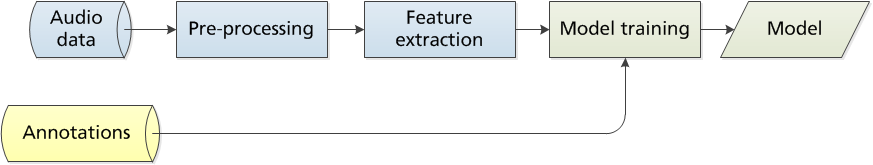
\includegraphics[width=1\textwidth]{figures/process_training.png}
                \caption{Schematic of the training procedure of the considered tasks.}
                \label{fig:process_training}
            \end{center}
        \end{figure}

        \begin{figure}
            \begin{center}
                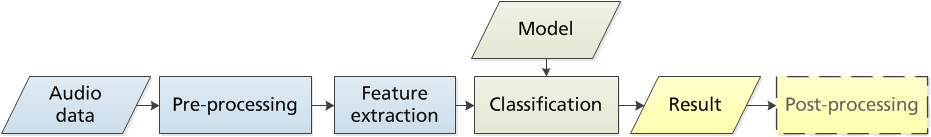
\includegraphics[width=1\textwidth]{figures/process_classification.png}
                \caption{Schematic of the classification procedure of the considered tasks (the model is the one created during training - see figure \ref{fig:process_training}).}
                \label{fig:process_classification}
            \end{center}
        \end{figure}

    \section{Feature Extraction}
        This section describes the Mel-Frequency Cepstral Coefficients (MFCCs) features. 
        MFCCs are among the most frequently used audio features in speech recognition. 
        They were first introduced in 1976 by Mermelstein and Davis \cite{mermelstein}\cite{davis_mermelstein} based on previous experiments by Bridle and Brown \cite{bridle_brown}.

        The basic idea behind MFCCs comes from experiments in human auditory perception. 
        Audio signals are transformed into a representation that is based on human perceptual sensitivities. 
        This is done by taking the Short-Term Fourier Transform (STFT) of an audio signal and then mapping the resulting spectrum from a linear frequency scale onto a Mel scale. 
        Then, the Discrete Cosine Transform (DCT) of the resulting log energies is calculated along the frequency axis to decorrelate the spectral band signals. 
        The result is a representation of the various frequencies within the spectrum (i.e. the cepstrum), which can be interpreted as ranging from the spectral envelope to the more fine-grained components. 
        In theory, this makes the result largely independent of the absolute frequencies (i.e. the pitch), but representative of the perceptual content (e.g. phonemes). 
        One point of criticism, however, is the lack of interpretability of the MFC coefficients.
        
        In detail, the calculation is performed as follows:

        \begin{description}
            \item[Short-term Fourier transform (STFT)] After cutting a signal $s$ into frames $s_i, i = 0,1,...,I$ (e.g. of 10ms duration) and windowing it (e.g. with a Hamming window), the Discrete Fourier Transform (DFT) is calculated for each time frame:
            \begin{equation}
                S_i(k) = \sum_{n=0}^{N-1} s_i(n)h(n)e^{-j 2\pi kn/N}, k = 0,1,...,K-1
            \end{equation}
            where $h(n)$ is the window of length $N$, and $K$ is the DFT length. For the further calculations, only the power spectrum is used:
            
            \begin{equation}
                P_i(k) = \frac{1}{N} \mid S_i(k) \mid ^2
            \end{equation}

            \begin{figure}
                \begin{center}
                    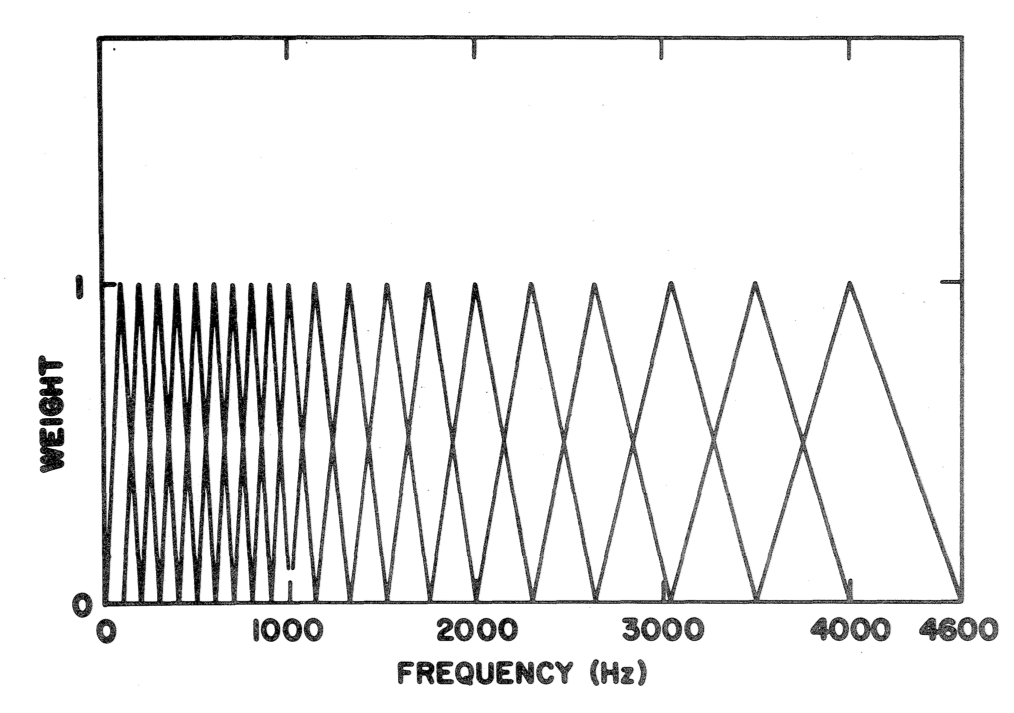
\includegraphics[width=0.6\textwidth]{figures/mel_filterbanks.png}
                    \caption{Example of a Mel filterbank. \cite{davis_mermelstein}}
                    \label{fig:mel_filterbanks}
                \end{center}
            \end{figure}

            \item[Mel-spectrum calculation] The resulting energies are mapped from the linear frequency scale to a perceptually motivated Mel scale. 
            This is done by convolving the spectrum with a set of $M$ triangular Mel-spaced filters $H_m(k)$, such as the ones shown in figure \ref{fig:mel_filterbanks}. 
            Furthermore, the resulting energy outputs are logarithmized:
            \begin{equation}
                X_m = \log_{10} \left( \sum_{k=0}^{K-1} \mid P_i(k) \mid \cdot H_m(k) \right), m=1,2,...,M
            \end{equation}

            \item[Discrete Cosine Transform (DCT)] Finally, the Mel-scale spectrum is transformed with a DCT, resulting in the so-called cepstrum:
            \begin{equation}
                C_j = \sum_{m=1}^{M} X_m \cdot \cos \left( (j+1) \cdot (m-1/2) \cdot \frac{\pi}{M} \right), j=0,1,...,J-1
            \end{equation}
            The $J$ MFC coefficients are retained as features. 
            The 0th coefficient can be interpreted as the power over all frequency bands, and the 1st coefficient as the global energy balance between low and high frequencies \cite{oshaughnessy}.
        \end{description}

        In addition, deltas and double-deltas are calculated to capture information about the feature's trajectory:
        \begin{equation}
            \Delta(C(n)) = C(n) - C(n-1) 
        \end{equation}
        \begin{equation}
            \Delta\Delta(C(n)) = \Delta(C(n)) - \Delta(C(n-1))
        \end{equation}

    \section{Deep Neural Networks} \label{sec:dnn}
        In recent years, Deep Learning has become the standard for machine learning applications \cite{schmidhuber_dl}. 
        This section also describes a new approach that was used extensively in this work: Deep Neural Networks (DNNs).

        \subsection{Artificial Neural Networks}
            \paragraph{History} Artificial Neural Networks have a long research history. 
            Based on an idea by McCulloch and Pitts from 1943 \cite{mcculloch_pitts}, they were slowly developed into functional algorithms for classification and pattern recognition. 
            Rosenblatt proposed a hardware design for a single-layer perceptron in 1958 \cite{rosenblatt}, while the first multi-layer networks were introduced by Ivakhnenko and Lapa in 1965 \cite{ivakhnenko}. 
            In 1969, Minsky and Papert posited many practical limitations for Neural Networks \cite{minsky_papert}, which led to a decrease in interest.

            The introduction of the backpropagation algorithm solved some of these issues and increased the training speed of multilayer networks \cite{werbos}, leading to a wider usage in speech recognition \cite{waibel_hanazawa} and other fields, such as computer vision \cite{srinivas} and Natural Language Processing \cite{goldberg}. 
            However, other algorithms such as SVMs began to produce better results over time and thus overtook Neural Networks in popularity.

            Over time, processing speed of computers increased, and better strategies and hardware for parallel computing became available. 
            This made the training of networks with many more layers possible, allowing for a much better adaptation to high-dimensional problems \cite{hinton_osindero}. 
            Over the past 10 years, this so-called ``Deep Learning'' has become the state of the art for many machine learning problems \cite{nytimes}\cite{schmidhuber_dl}\cite{deng_hinton_kingsbury}.

            \paragraph{Functionality} Artifical Neural Networks (ANNs) are inspired by ``real'' Neural Networks - i.e. the human brain and nervous system. 
            They consist of neurons, which are nodes that can process inputs and send outputs, and the connections between them. 
            These neurons are grouped in layers: An input layer, an output layer, and a number of hidden layers in between them. 
            Historically, ANNs had no hidden layers at all; this type of ANN was called ``perceptron''. 
            Later, hidden layers were introduced and the resulting networks were called ``Multilayer Perceptrons'' (MLPs).
            
            Networks with no hidden layers are only able to solve linear problems; the introduction of hidden layers added non-linear projections to the calculation. 
            Recent ``Deep'' Neural Networks (DNNs) possess more hidden layers, leading to an exponential increase of the degrees of freedom and thus the possibility to model much more complex problems.

            \begin{figure}[htbp]
                \centering
                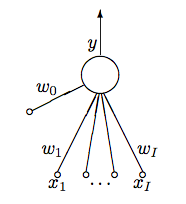
\includegraphics[width=0.2\textwidth]{figures/neuron.png}
                \caption{Functionality of a single neuron in an ANN. The neuron computes a weighted sum of its inputs, and then applies an activation function, resulting in output $y$. \cite{mackay}}
                \label{fig:neuron}
            \end{figure}


            \begin{figure}
                \centering
                \begin{subfigure}[t]{0.3\textwidth}
                    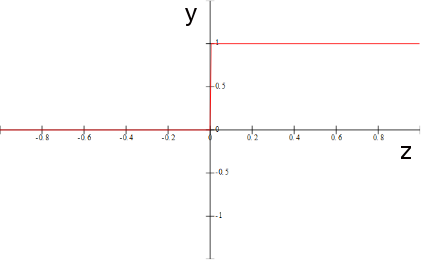
\includegraphics[width=\textwidth]{figures/activation_heaviside.png}
                    \caption{Heaviside binary step}% activation function}
                    \label{fig:activation_heaviside}
                \end{subfigure}
                \begin{subfigure}[t]{0.3\textwidth}
                    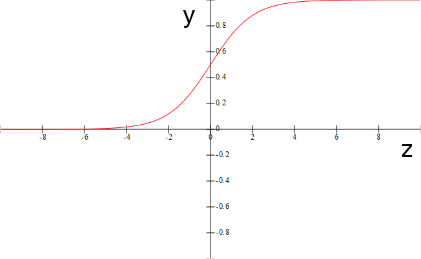
\includegraphics[width=\textwidth]{figures/activation_sigmoid.png}
                    \caption{Sigmoid}% activation function}
                    \label{fig:activation_sigmoid}
                \end{subfigure}
                \begin{subfigure}[t]{0.3\textwidth}
                    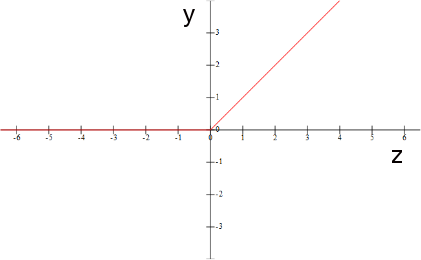
\includegraphics[width=\textwidth]{figures/activation_relu.png}
                    \caption{ReLU}% activation function}
                    \label{fig:activation_relu}
                \end{subfigure}
                \caption{Activation functions used for ANN neurons. \cite{medium}}
            \end{figure}
                  
               
            The function of a single neuron is visualized in figure \ref{fig:neuron}. 
            Classic neurons compute a weighted sum $z$ of their inputs $x = (x_1,x_2,...,x_I)$:
            \begin{equation}
                z = w_0 + \sum_{i=1}^I x_i w_i = w_0 + w^\top x
            \end{equation}

            where $w = (w_1,w_2,...,w_I)$ is a vector of weights, and $w_0$ is a constant bias. 
            This result is often called the ``logit''. 
            Then, a nonlinear activation function can be applied. 
            In perceptrons, this was the Heaviside step function, shown in figure \ref{fig:activation_heaviside}, resulting in a binary output:
            \begin{equation}
                y = \begin{cases}
                    1 \text{ if } z \leq 0\\
                    0 \text{ otherwise}
                \end{cases}       
            \end{equation}

            An activation function commonly used is the sigmoid function, shown in figure \ref{fig:activation_sigmoid}:
            \begin{equation}
                y = \frac{1}{1 + e^{-z}}
            \end{equation}

            Neurons of this type are called ``logistic'' neurons. 
            This function is often applied because it generates a smooth, real-valued output and has easy-to-use derivatives, simplifying the training process.

            Rectified linear units (ReLUs) are also used frequently since they train faster than logistic units and retain more information that is relevant in the middle layers (in particular, this leads to sparsity for small inputs and a lower risk of vanishing or exploding gradients). 
            The function is shown in figure \ref{fig:activation_relu}:
            \begin{equation}
                y = \max(0, z)
            \end{equation}

            In the last layer, a so-called softmax activation function is often applied. 
            This function takes the outputs of all neurons into account, and computes a probability distribution (i.e. all the outputs will sum up to one and represent the likelihood of the corresponding class):
            \begin{equation}
                y_j = \frac{e^{z_j}}{\sum_{k=1}^M e^{z_k}}, 1 \leq j \leq M
            \end{equation}

            where $M$ is the number of output neurons.

            \paragraph{Training} Neural Network training is nowadays usually performed via the backpropagation algorithm. 
            This algorithm is based on the calculation of a cost (or error) function $E$, which computes the difference between the network output and the expected output (e.g. the annotated classes in the training data). 
            Then, the partial derivatives of the cost are calculated with regards to the weights, using the outputs and logits for the chain rule:
            \begin{equation}
                \frac{\partial E}{\partial w_{ij}} = \frac{\partial E}{\partial y_j} \frac{\partial y_j}{\partial z_j} \frac{\partial z_j}{\partial w_{ij}}
            \end{equation}

            Then, the weights are adjusted accordingly:
            \begin{equation}
                \Delta w_{ij} = - \eta \frac{\partial E}{\partial w_{ij}}
            \end{equation}

            where $\eta$ is the so-called learning rate, which must be chosen carefully to ensure convergence of the training process. 
            In the same way, the error is propagated further backwards through the model to adjust the weights of the previous layers. 
            This is done until all the weights have been adjusted. 
            Then, the next batch of training data is passed through the model and the process is repeated. 
            The training process is performed until the weights converge (or until a fixed number of iterations has been reached).

            A commonly used cost function is the squared error measure (employing the $L^2$ or Euclidean norm):
            \begin{equation}
                E_S = \frac{1}{2} \sum_{j=1}^{M} (t_j - y_j)^2
            \end{equation}

            where $t_j$ is the target value for output unit $j$. 
            Alternatively, the cross-entropy is often chosen as the cost function when using a softmax output layer:
            \begin{equation}
                E_C = - \sum_{j=1}^M t_j \log y_j
            \end{equation}

            \paragraph{Curse of dimensionality} One of the major issues in Neural Networks is that of overfitting: 
            The model adapts too well to the training data and is not able to sufficiently generalize to new data anymore. 
            This is especially relevant for deep networks because of the many degrees of freedom.

            There are several strategies to overcome this problem. One of the most frequently used regularization techniques is dropout: 
            During training, nodes in the network are deactivated randomly, effectively resulting in many different network structures and making the whole network robust to variations in the data. 
            The most crucial point, however, is the amount of data used for training the network. 
            The more variety is available, the lower the risk of overtraining.

            The so-called ``curse of dimensionality'' is a concept that applies to many machine learning algorithms. 
            However, Goodfellow et al. make an argument that deep models operate on a different level altogether \cite{goodfellow}: 
            Where traditional machine learning methods make an assumption of smoothness of the hidden functions to be represented, deep models actually attempt to model the underlying structures in a distributed way. 
            This means that information about outputs can be learned in a shared way - i.e., if two classes have something in common, the model is also able to represent this fact. 
            Practically, the many degrees of freedom do not lead to ``learning by heart'', but instead allow for an internal representation of highly complex relationships. 
            Goodfellow et al. mention two interpretations of the deep modeling capabilities: 
            Learning a representation composed of simpler representations (e.g. corners defined by edges), or learning sequential steps that build on top of each other (e.g. first locate objects, then segment them, then recognize them). 
            There is also a number of publications that demonstrate better generalization abilities for deeper networks \cite{bengio07}\cite{bengio09}\cite{ciresan}\cite{erhan09}\cite{krizhevsky}\cite{szegedy}. 
            In an experiment in \cite{goodfellow_experiment}, models with three hidden layers overfit at 20 million parameters, while a deep model (11 hidden layers) benefits from more than 60 million. 
            This is because a deep model has the capability to learn the actual explanatory factors behind the expected outputs (e.g. learning about different genders or whether a person is wearing glasses when modeling faces \cite{radford}).

            \paragraph{Types} In addition to the various types of neurons, ANNs themselves can be grouped into different types. 
            In their basic configuration, ANNs will have multiple layers of the described neurons where connections are only allowed in one direction. 
            A schematic is shown in figure \ref{fig:feedforward}. 
            This type of network is called ``feed forward'' or, in the context of Deep Learning, a Deep Neural Network (DNN). 
            In this work, DNNs with logistic units in the hidden layers and a softmax output layer were used in phoneme classification tasks.

            \begin{figure}[htbp]
                \centering
                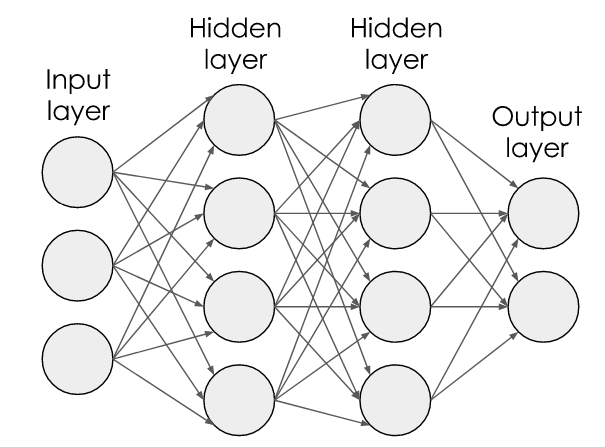
\includegraphics[width=0.4\textwidth]{figures/feedforward.png}
                \caption{Schematic of a feed-forward neural network with an input layer with three neurons, two hidden layers with four neurons each, and an output layer with two neurons. \cite{medium}}
                \label{fig:feedforward}
            \end{figure}

            If connections that skip back are allowed in the network, the network is called a Recurrent Neural Network (RNN). 
            These networks are particularly useful for modeling time-dependent series because they have the ability to ``store'' temporal states in their units. 
            However, they were deemed impractical for a long time because they exhibit the exploding/vanishing gradient problem during training \cite{Hochreiter1998}. 
            This problem was solved with the introduction of memory cells in place of neurons, in particular Long Short-Term Memory (LSTM) units \cite{Hochreiter1997} and Gated Recurrent Units (GRU) \cite{Cho2014}. 
            Nowadays, RNNs are being used successfully in a number of research tasks \cite{lstm_sak_senior}.

            Another type of Neural Network are Convolutional Neural Networks (CNNs). 
            These networks add layers of filters (so-called convolutional layers) before or in between classic fully-connected layers. 
            The parameters of these filters are trained jointly with the other layers. For this reason, CNNs are able to ``learn'' a feature representation of the input. 
            They were first used in image recognition \cite{krizhevsky}, but are now also being used for audio-related tasks such as environmental sound classification \cite{piczak} and ASR \cite{abdelhamid}. 
            A disadvantage of both RNNs and CNNs is the computational complexity of training them, and the requirement for even more training data because they possess even more degrees of freedom than DNNs of comparable sizes.

        \subsection{Convolutional Neural Networks}

            The neural network or multi-layered network of neurons can learn the relation between the input and output using non-linear mapping function. 
            But in the case of images, a neural network would, for a given task, take into account the entire image. 
            This, in turn, makes the neural network highly inefficient in terms of pragmatic quality as well as neural network quality, as, the number of parameters to learn increases. 
            Hence, to solve this problem, another type of neural network called Convolution Neural Networks is used, which is specifically designed for computer vision-related tasks such as image classification, semantic segmentation, object detection, etc.

            The inception of CNNs happened in the year 1960 by D.H Hubel and T.N Wiesel in their paper \cite{hubel1962receptive} where they described two types of cells in the human brain (specifically in the visual cortex), simple cells, and complex cells. 
            Simple cells are activated when they identify basic shapes in a fixed area and a definite angle. 
            The complex cells have bigger receptive fields, and their output is not sensitive to specific positions in the field. 
            Taking inspiration from \cite{hubel1962receptive}, in the year 1998, CNNs was re-introduced in the paper \cite{lecun1998gradient} called LeNet-5 which was able to classify digits from hand-written numbers. 
            Since it's inception to the present era, the CNNs has been used in various state of the art applications, especially in the field of computer vision.

            There are four main operations in CNNs. 
            Figure \ref{fig:convolution_layer} shows how all the components are linked to each other in a CNN.
            These operations are the essential building blocks in every CNNs:
            \begin{itemize}
                \item Convolution operation
                \item Activation
                \item Pooling
                \item Fully-connected layer
            \end{itemize}

            \begin{figure}[h!]
                \centering
                    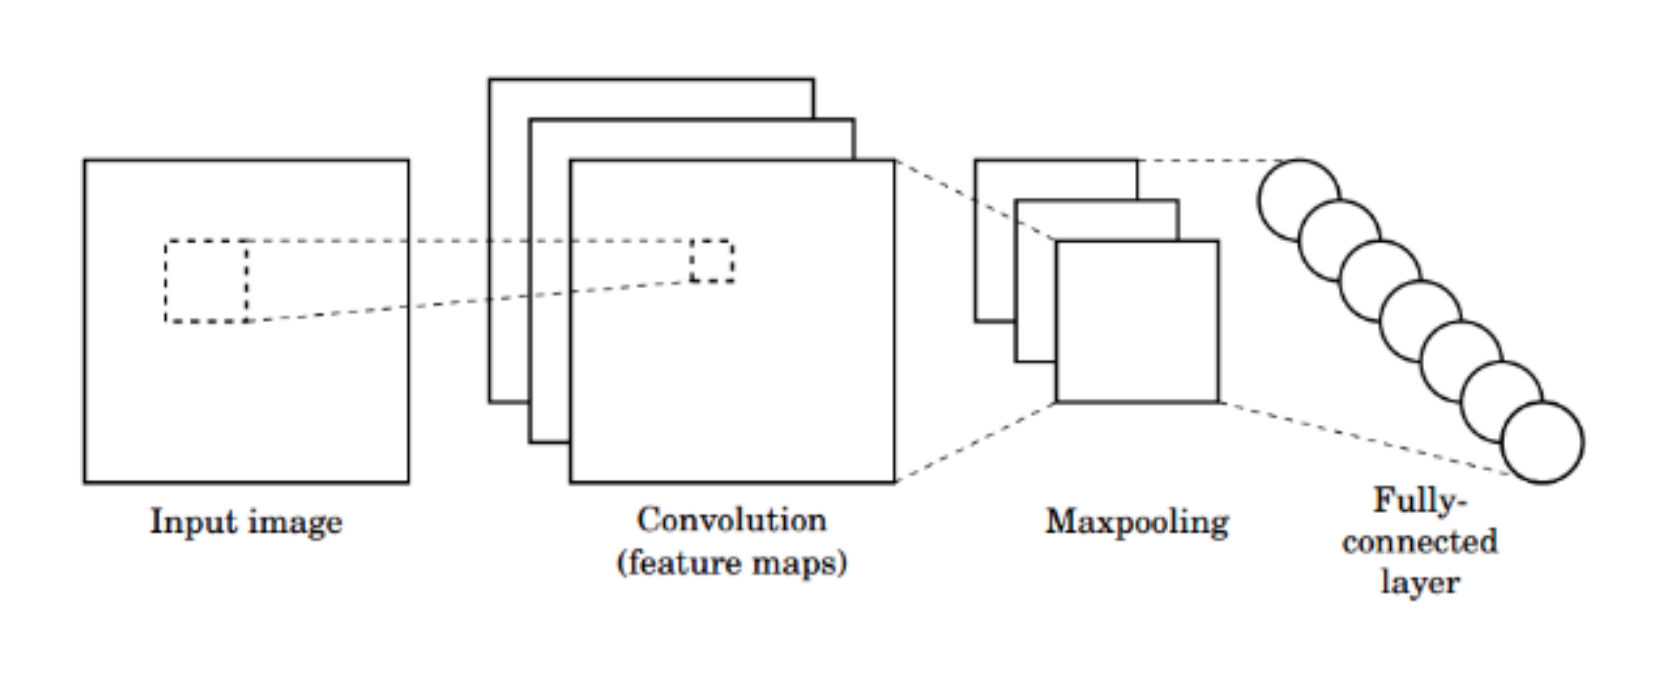
\includegraphics[width=\linewidth]{figures/convolution_layer.png}
                \caption{Components of a CNN}
                \label{fig:convolution_layer}
            \end{figure}

            \begin{figure}[h!]
                \centering
                    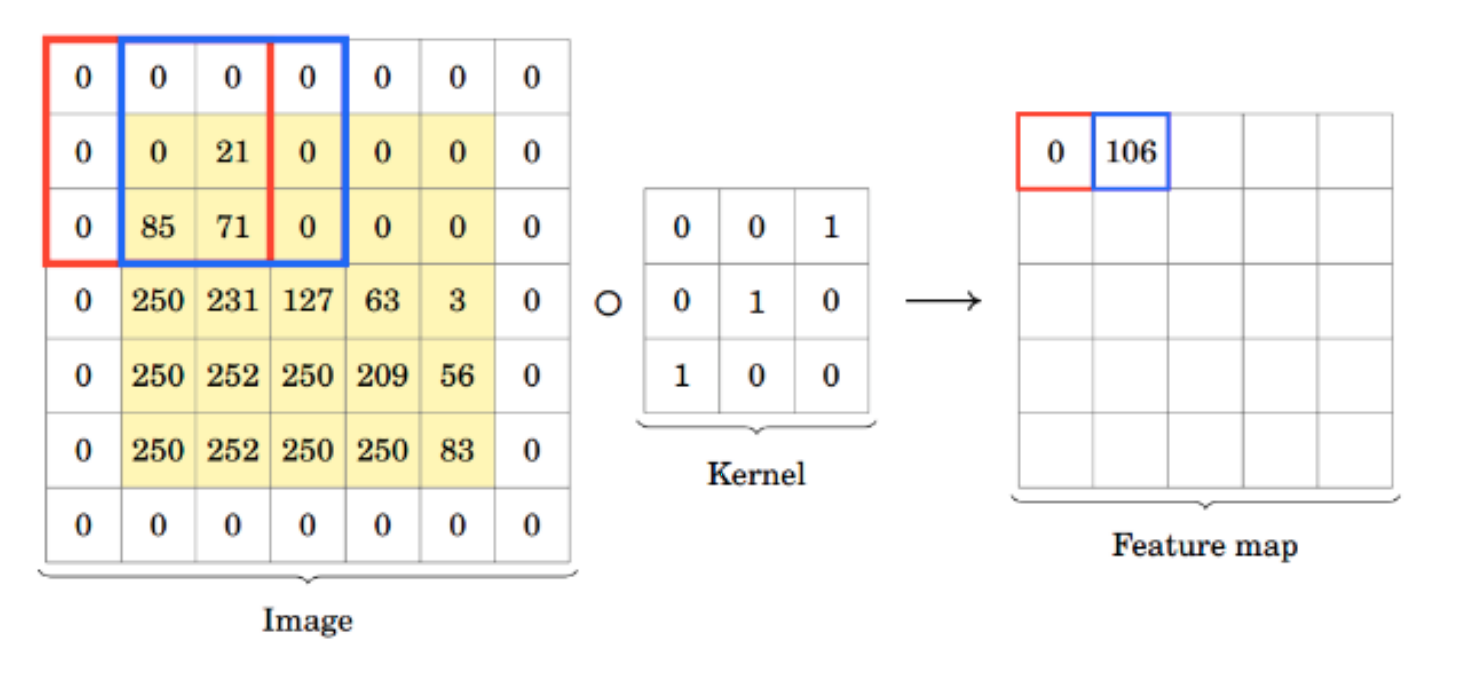
\includegraphics[width=0.8\linewidth]{figures/convolution_operation.png}
                \caption{A convolution operation \cite{VoPa}}
                \label{fig:convolution_operation}
            \end{figure}

            \paragraph{Convolution operation} Consider the example on figure \ref{fig:convolution_operation} showing how the convolution works. 
            There is an image (x) of \textit{7$\times$7} and a kernel or filter (k) of \textit{3$\times$3}.
            Slide the filter over the image pixel-by-pixel and for every position and compute the element-wise multiplication between the two matrices and then, add the outputs to get a final integer which forms a single element in the output matrix. 
            The output matrix is so-called an activation map or feature map. 
            Hence, a CNN investigates only a piece of the image rather than the entire image at once, making it different from other neural networks. 

            A convolution neural network learns the values (weights) of the filters on its own during the training process. 
            CNNs can have multiple numbers of filters such that more features from the image get extracted, and better the network becomes in observing and recognizing patterns. 
            
            The size of the feature map can be controlled by three parameters, they are:
            \begin{itemize}
                \item Depth - This is the number of filters we use for the convolution operation. 
                For example, if we use three distinct filters on the input image, we will have three feature maps that are stacked together. 
                
                \item  Stride - It determines the number of pixels by which the filter slides over the input matrix. 
                For example, if the stride value is 1, we move the filter over the input by one pixel at a time. 
                If the stride value is 3, we move the filter over the input by jumping 3 pixels at a time.
                
                \item Zero-padding - We pad the input matrix with zeros around the border such that filter can be applied to the bordering elements of the input matrix. 
                Applying zero-padding is called as wide-convolution and not using zero-padding is called as narrow-convolution.
            \end{itemize}

            \paragraph{Activation} The non-linear activation functions are responsible for the model to create complex mappings between the input and the output such that modeling complex data such as images, videos, audios, which are, high dimensional in nature is possible. 

            \paragraph{Pooling} Pooling step is done to reduce the dimensionality of the feature map and preserve the most important features from the map. 
            This process is also called as downsampling of upsampling.
            Pooling has further advantages like:
            \begin{itemize}
                \item It makes the input representations smaller and hence, more manageable.
                \item It reduces the number of parameters and therefore, controls overfitting.
                \item It makes the model unvaried to small distortions, translations in the input image.
                \item It makes an invariant representation of the image due to which, the network can detect objects at any located position in the image. 
            \end{itemize}

            There are three types of pooling: 
            \begin{itemize}
                \item Max pooling - Define a spatial neighbourhood $2\times2$ window and take the largest element from each window of the feature map to form a new output matrix. 
                Figure \ref{fig:maxpool} shows how max-pooling works. 
                
                \item Average pooling - Define a spatial neighbourhood $2\times2$ window and take the average of all the elements in each window from the feature map, to form a new output matrix with the average values.
                
                \item Sum pooling - Define a spatial neighbourhood $2\times2$ window and take the sum of all the elements in the window from the feature map, to form the new output matrix with the sum values.
            \end{itemize}
            
            \begin{figure}[h!]
                \centering
                    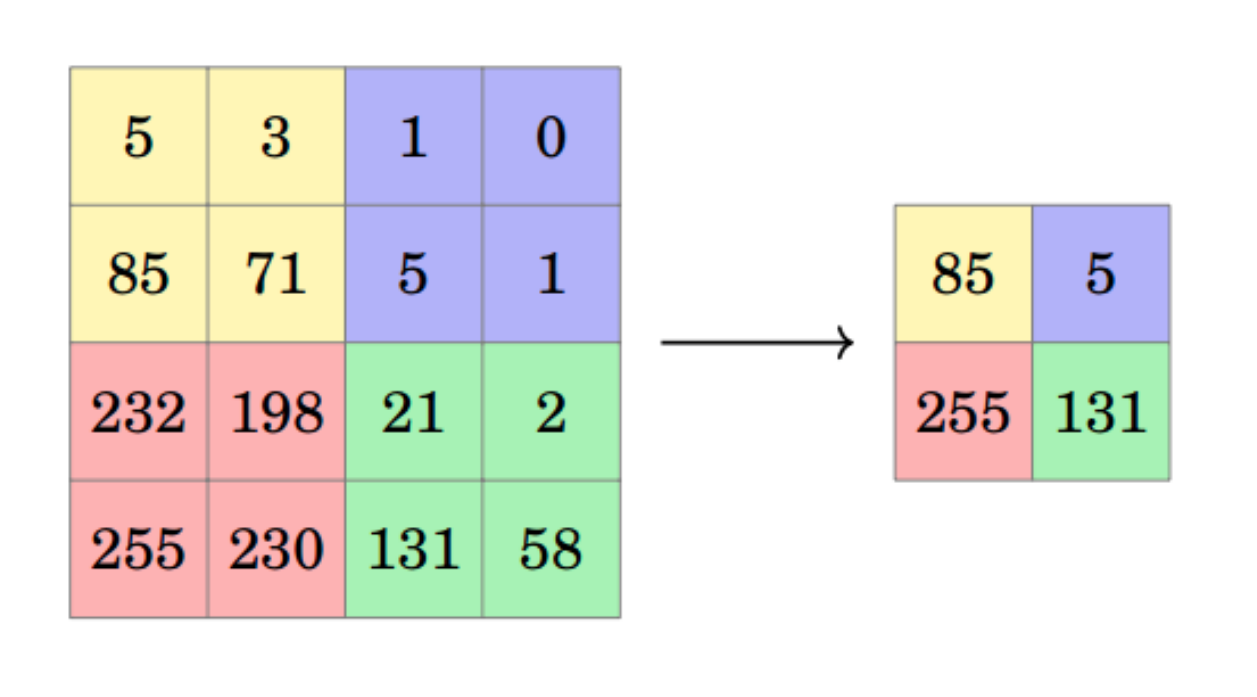
\includegraphics[width=0.4\linewidth]{figures/maxpooling.png}
                \caption{Max-pooling operation}
                \label{fig:maxpool}
            \end{figure}

            \paragraph{Fully connected layer} The term 'fully connected' implies that every neuron in the layer is connected with the neurons of the previous layer. 
            The convolutional layers and pooling layers are used to extract features from the input image, while the fully connected layer uses these extracted features to classify the input image into separate classes based on the training dataset. 
            A softmax function is used as the activation function in order to get the probabilities of each class in the dataset. 

        \subsection{Recurrent Neural Networks}

            A recurrent neural network (RNN) is rather similar to a multilayer perceptron, but it takes previous inputs into account. 
            The input to an RNN is a sequence of samples. 
            An RNN can be used for other tasks where the order of samples are important, e.g. time series forecasting or natural language processing.
            Recurrent neural networks stores hidden representations of inputs and conveying that information to the next input in the sequence \cite{Goodfellow-et-al-2016}. 

            \begin{figure}[t]
                \centering
                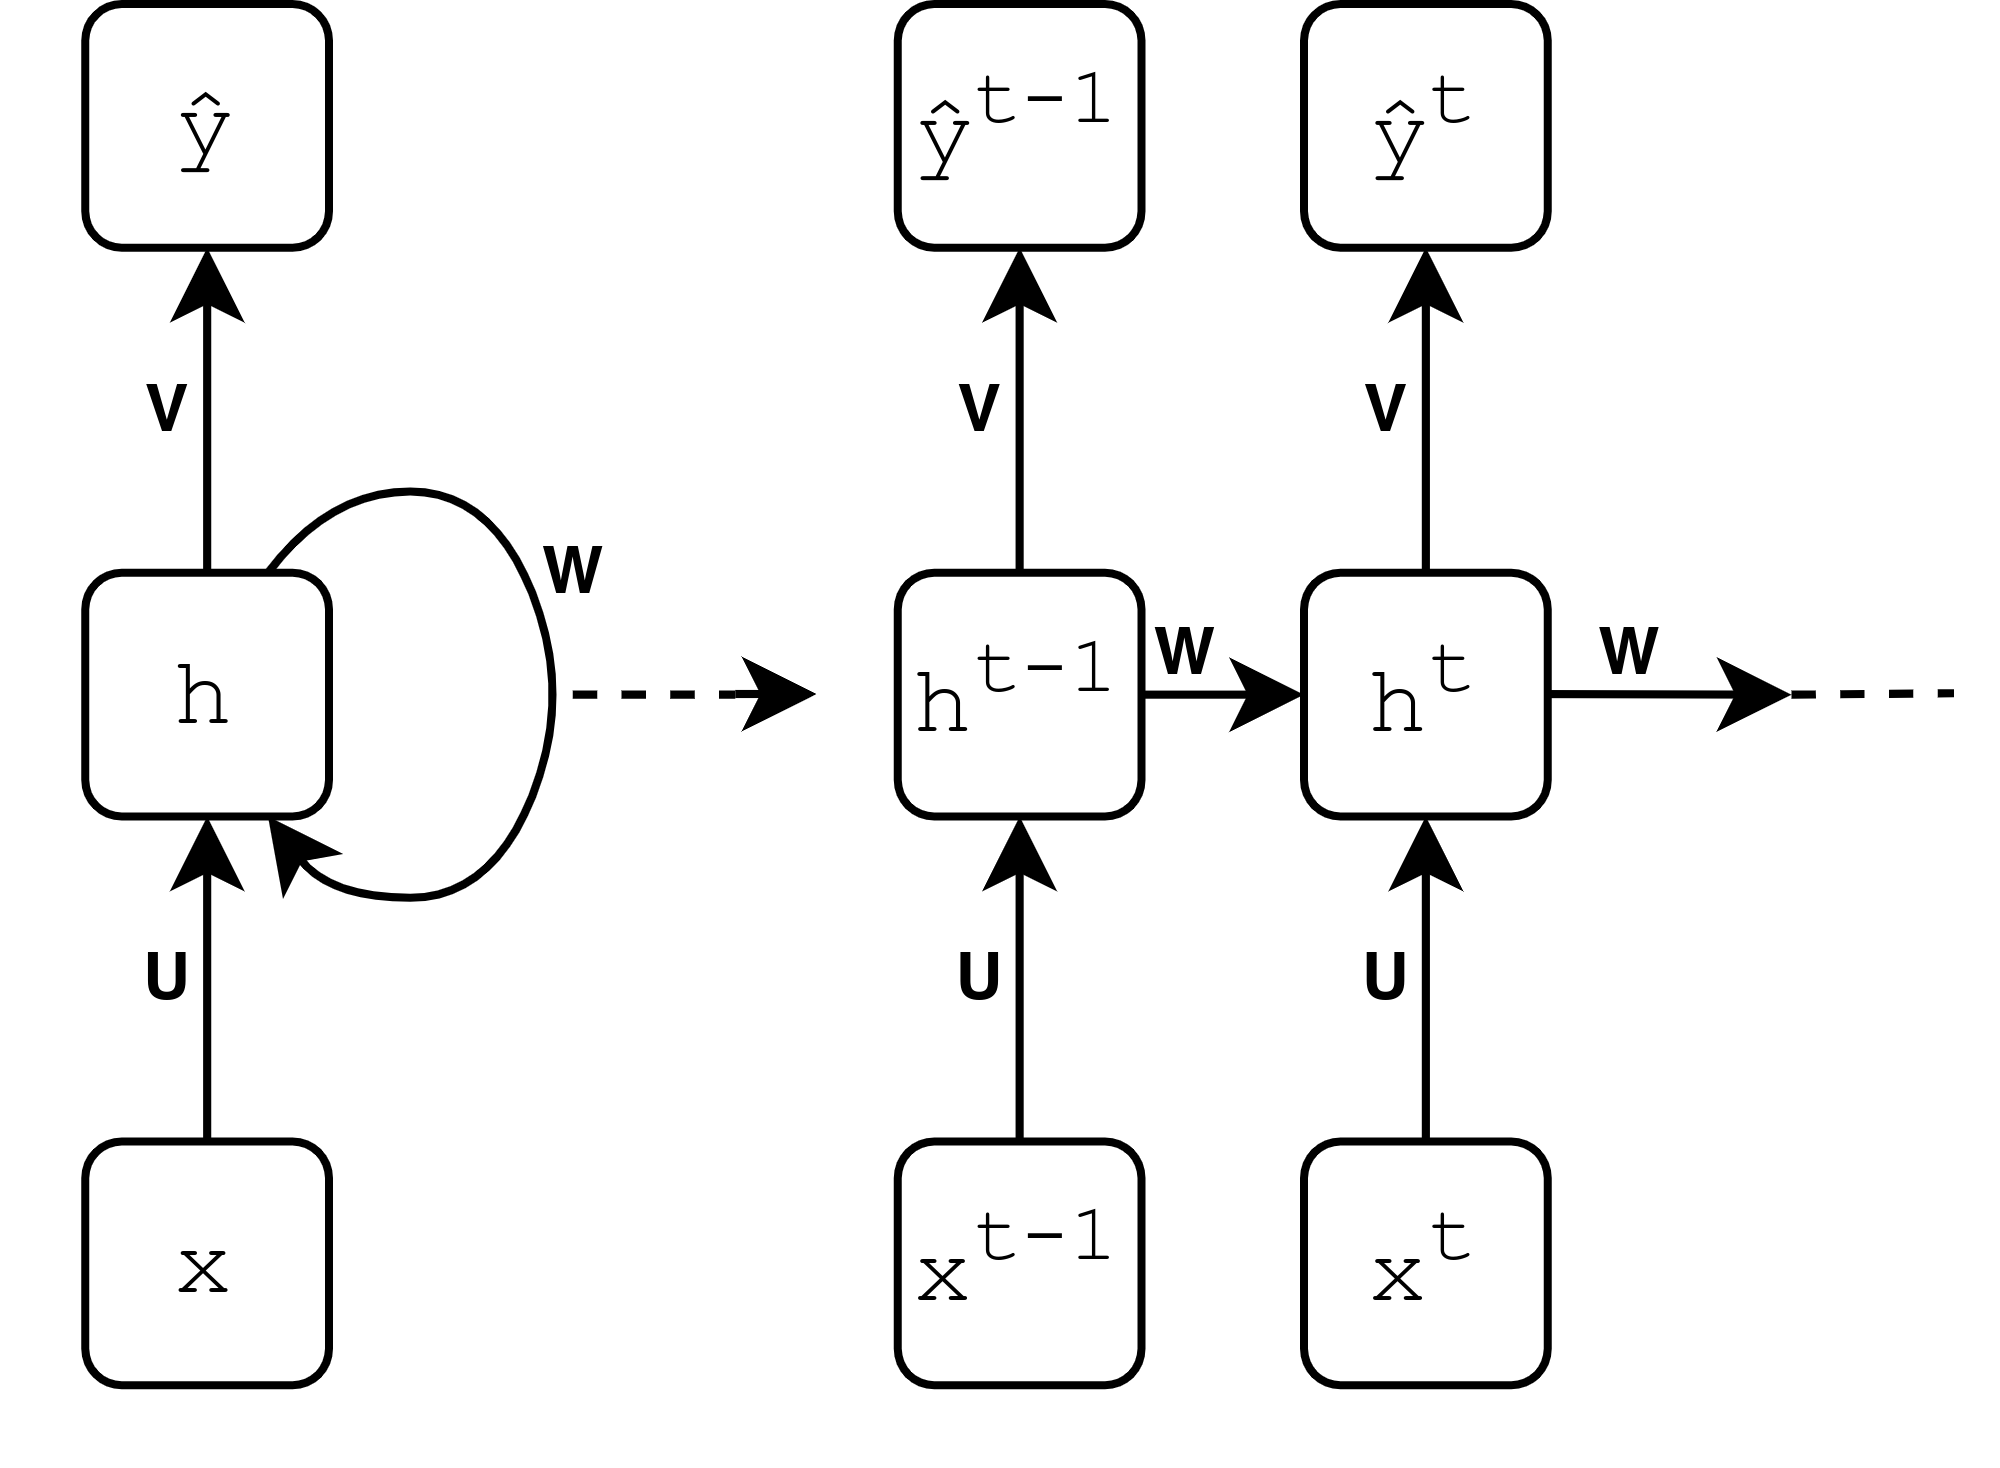
\includegraphics[width=0.5\textwidth]{figures/simple_rnn.png}
                \caption{General graph of a sequence-to-sequence RNN unfolded through time, where a sequence of inputs $x$ predicts a sequence of outputs $y$. $\mathbf{U}$, $\mathbf{V}$ and $\mathbf{W}$ are weights that are shared throughout the sequence, independent of the position.}
                \label{fig:rnn}
            \end{figure}

            As seen in figure~\ref{fig:rnn}, an RNN can be seen as a feed-forward neural network where previous time steps are used as input. 
            Assuming a hidden layer activation function $\sigma_h$ and an output activation function $\sigma_o$, the recurrent nature of the model can be further explained. 
            Let the other notation be as in figure~\ref{fig:rnn}. 
            \begin{equation}
                \hat{y_t} = \sigma_o(V \cdot h^{(t)}) = \sigma_o(V \cdot  \sigma_h(U x^{(t)} + W h^{(t-1)}))
            \end{equation}

            \begin{equation}
                h^{(t-1)} = \sigma_h(Ux^{(t-1)} + W h^{(t-2)})
            \end{equation}


            Clearly, the prediction $\hat{y}^{(t)}$ is dependent on the previous inputs $x^{(i)}$ and hidden states $h^{(i)}$. 
            The model structure is similar for sequence-to-one classifications, i.e. a sequence $(x_i^{(1)}, x_i^{(2)}, ..., x_i^{(l)})$ predicts one label $\hat{y}_i$. 
            Given a sequence length $l$, only the final step $x_i^{(l)}$ provides an output $y_i$. 
            This output is however influenced by the previous inputs $x_i^{(t)}$ through the hidden layers $h^{(t)}$ and the weights $W$, see Figure~\ref{fig:rnns2o}. 

            \begin{figure}[t]
                \centering
                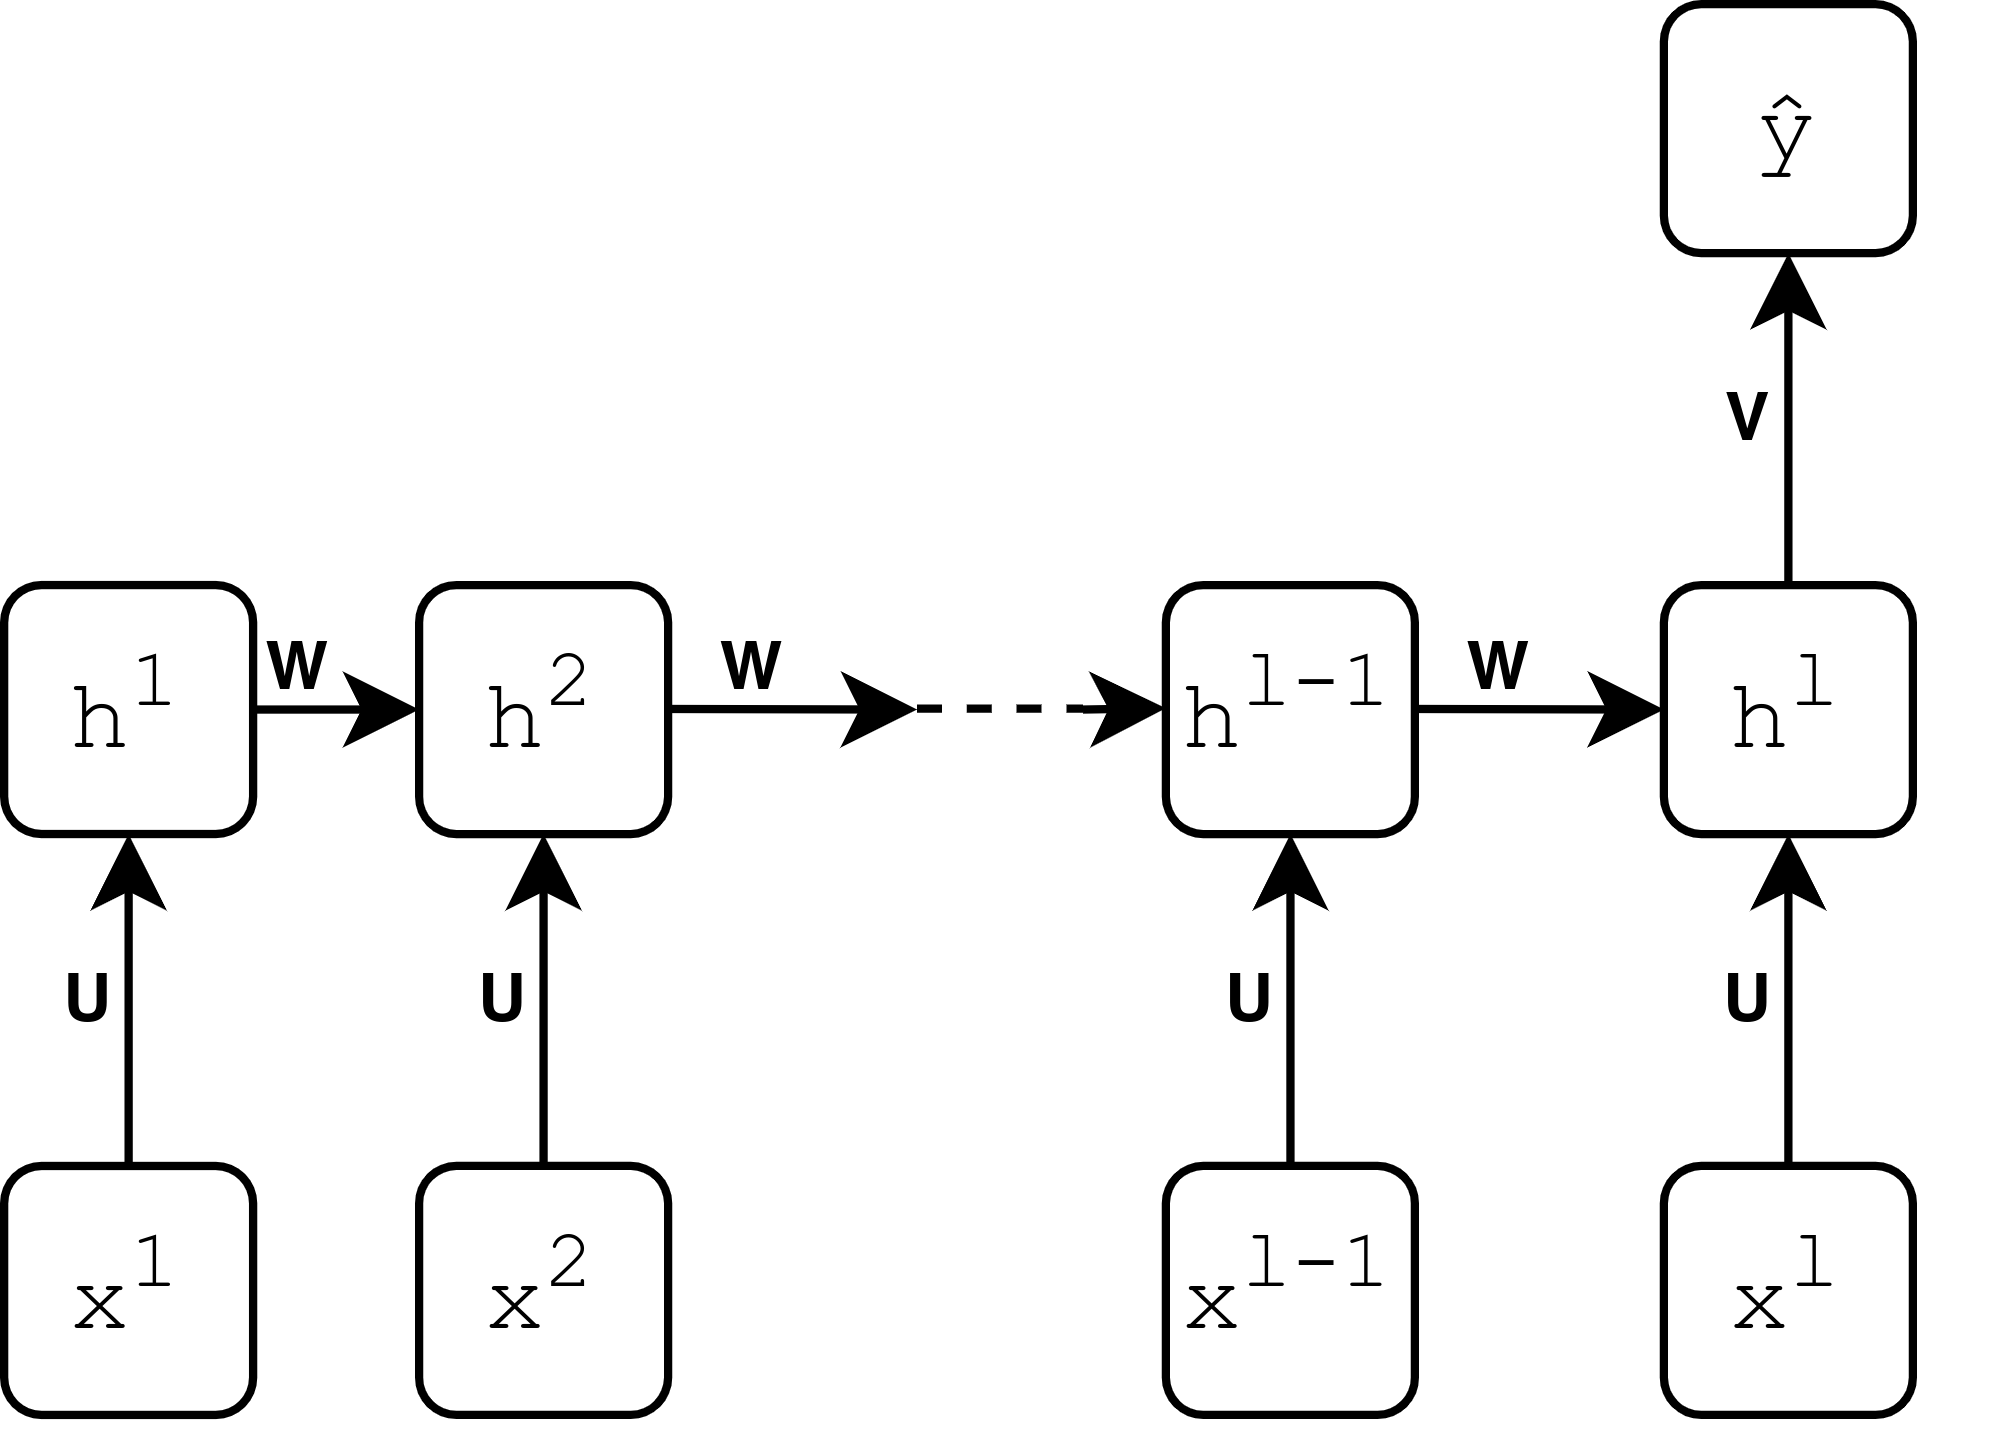
\includegraphics[width=0.5\textwidth]{figures/rnn-s2o.png}
                \caption{Schematic graph of a sequence-to-one RNN unfolded through time, where a sequence of inputs $(x^{(1)}, ..., x^{(l)})$ predicts one output $y$.}
                \label{fig:rnns2o}
            \end{figure}

            Even though the general idea of the previously described method is widely used, the model is not used precisely as described. 
            The simple RNN-structure suffers from the \textit{vanishing gradient problem}. 
            To understand this problem, one must understand how the network is trained, which is outside the scope of this report. 
            In short, long term dependencies are too many time-steps away to have an impact when the network is trained. 

            In practice, either Long-Short-Term Memory (LSTM) or Gated Recurrent Unit (GRU) are used instead. 
            The main difference is that information that is deemed important is allowed to pass on to later time-steps without too much interference from hidden several dot products and activation functions. 
            This alleviates the vanishing gradient problem, even though the core idea is the same as the previously described simple RNN \cite{chollet2017deep}.


            \paragraph{Long Short-Term Memory (LSTM)} The LSTM architecture, contrary to regular RNNs, has an additional hidden state that is never directly outputted (see Figure~\ref{fig:lstm_cell}). 
            This additional hidden state can then be used by the network solely for remembering previous relevant information. 
            Instead of having to share its ``memory'' with its output, these values are now separate. 
            During the training process, an LSTM learns what should be remembered for the future and what should be forgotten, which is achieved by using its internal weights.

            \begin{figure}[h!]
                \begin{center}
                    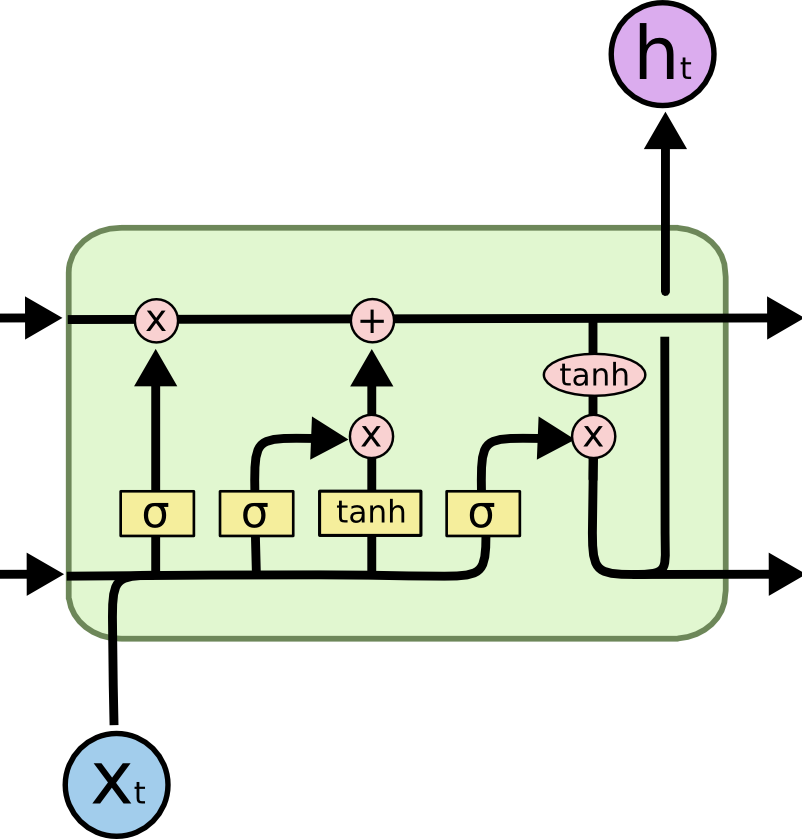
\includegraphics[scale=0.5]{figures/lstm_cell.png}
                \end{center}
                \caption{A single LSTM cell. From~\cite{olah2015understanding}\label{fig:lstm_cell}}
            \end{figure}

            As can be seen in the figure, there are quite a few more parameters in this cell than in a normal RNN cell. 
            The calculation of the output vector and the hidden vector involves several operations, a full explanation of which can be found in~\cite{olah2015understanding}. 
            First of all the network determines how much of the hidden state to forget, also called the forget gate. 
            This is done by pushing both the previous iteration's output (\(c_{t-1}\)) and the forget gate vector (\(f_t\)) through a matrix multiplication. 
            This allows the network to forget values at specific indices in the previous iteration's output vector. 
            \(f_t\) can be obtained by using formula~\ref{eq:forget_vector_lstm}, where \(W\) contains the weights for the input and \(U\) contains the weights for the previous iteration's output vector, \(x_t\) refers to the input, \(h_{t-1}\) to the previous iteration's output vector and \(b\) to a set of bias vectors:
            \begin{equation} \label{eq:forget_vector_lstm}
                f_t = \sigma(W_f x_t + U_f h_{t-1} + b_f)
            \end{equation}

            The network then determines what to remember from the input vector.
            This is commonly referred to as the input gate. 
            This is done by pushing the previous forget gate's output as well as the input gate through a matrix addition function. 
            The output of the input gate (\(i_t\)) can be found by using the following formula:
            \begin{equation} \label{eq:input_vector_lstm}
                i_t = \sigma(W_i x_t + U_i h_{t-1} + b_i)
            \end{equation}

            The final hidden state vector (\(c_t\)) can then be found by using the previous two results as follows, where \(\circ \) denotes the Hadamard product (where each value at index \(ij\) is the product of the values at the indices \(ij\) in the two input matrices): 
            \begin{equation} \label{eq:hidden_state_vector_lstm}
                c_t = f_t \circ c_{t-1} + i_t \circ \sigma(W_c x_t + U_c h_{t-1} + b_c)
            \end{equation}

            This vector is then passed on to the next iteration. 
            Now the output gate vector \(o_t\) is calculated:
            \begin{equation} \label{eq:output_gate_lstm}
                o_t = \sigma(W_o x_t + U_o h_{t-1} + b_o)
            \end{equation}

            The output state \(h_t\) can then be obtained:
            \begin{equation} \label{eq:hidden_output_gate_lstm}
                h_t = o_t \circ \sigma(c_t)
            \end{equation}

            This results in a version of an RNN that is able to remember more and is more liberal in choosing what information it wants to keep in the hidden state and what it wants to discard. 
            This makes LSTM networks better suited for tasks involving series of data. 
            This has lead to the LSTM architecture becoming the dominant RNN architecture. 

            \paragraph{Gated Recurrent Units (GRUs)} Another RNN architecture is the Gated Recurrent Unit (GRU), introduced in~\cite{cho2014learning}. 
            This architecture combines the input and forget gates into a single so-called ``update gate'' and also merges the cell state and hidden state (see Figure~\ref{fig:gru_cell}). 
            The calculation of the merged output vector once again consists of several operations. The network first computes the ``reset gate'' \(r_t\) using the following function, where \(W_r\) are the weights for the reset gate and \([h_{t-1}, x_t]\) signifies the concatenation of \(h_{t-1}\) and \(x_t\):

            \begin{figure}[h!]
                \begin{center}
                    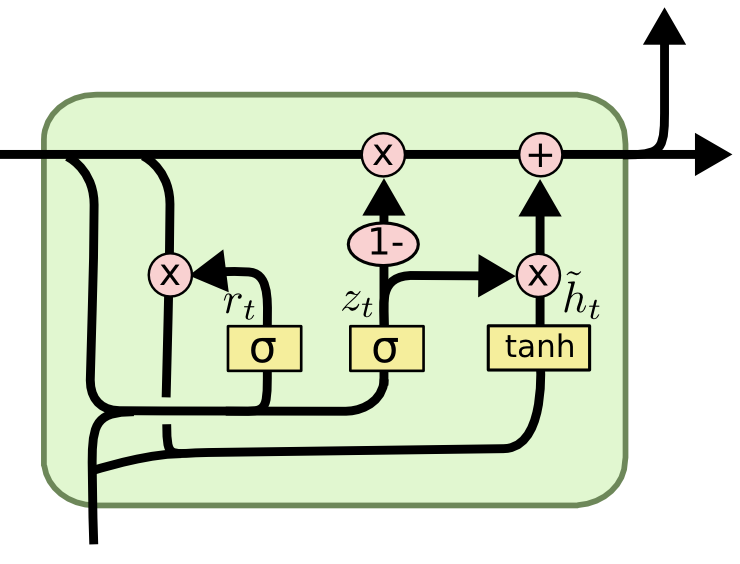
\includegraphics[scale=0.5]{figures/gru_cell.png}
                \end{center}
                \caption{A single GRU variation cell. From~\cite{olah2015understanding}\label{fig:gru_cell}}
            \end{figure}

            \begin{equation} \label{eq:gru_reset_gate}
                r_t = \sigma(W_r [h_{t-1}, x_t])
            \end{equation}

            After this, the ``update gate'' \(z_t\) is computed as follows, where \(W_z\) holds the weights of the update gate:
            \begin{equation} \label{eq:gru_update_gate}
                z_t = \sigma(W_z [h_{t-1}, x_t])
            \end{equation}

            The output vector \(h_t\) (representing both the cell's output and its state) can then be computed by the following function:
            \begin{equation} \label{eq:gru_output}
                h_t = (1 - z_t) * h_{t-1} + z_t * \tilde{h_t}
            \end{equation}

            Where \(\tilde{h_t}\) is computed by:
            \begin{equation} \label{eq:gru_output_partial}
                \tilde{h_t} = \tanh(W * [r_t * h_{t-1}, x_t])
            \end{equation}

            \paragraph{Bidirectional RNNs} It should be mentioned that when RNNs are used, they are often wrapped with a bidirectional layer.
            This simply reverts the input sequence and enters the sequence in both the original and the reverse direction to two separate RNNs, usually LSTM or GRU. 
            The usefulness of this is particularly intuitive when looking at the network in Figure~\ref{fig:rnn}. 
            When processing the entry $x^{(j)}$, only the entries $t < j$ are known. 
            However, tokens later in the sequence might have an impact on the previous outputs of the model. 
            Bidirectional RNNs can catch patterns that are overlooked by regular RNNs.

    % !TEX root = ../main.tex
\chapter{Related Works} \label{chap:related_works}

    \section{Introduction}\label{sec:related_intro}

        The aim of KWS is to detect specific keywords/key-phrases in an audio stream, and there are several conventional KWS systems.
        For example, dynamic time warping (DTW) based KWS searches for matches between a sliding window of speech signal and the template of the keyword based on the DTW algorithm \cite{SC78}.
        Large-vocabulary continuous speech recognition (LVCSR) based KWS first utilizes a LVCSR system to transcribe the input audio stream into text or rich lattices, then employs efficient searching algorithms to determine the position of the keyword in the text or lattices \cite{GAV00,MKK+07}.
        Another widely used KWS approach is the Keyword/Filler HMM-based KWS; for each predefined keyword, this approach trains an HMM on a training dataset, and a filler HMM is trained for all non-keywords speech, noise, and silence \cite{RRRG89,RP90,WMM91}.
        Both LVCSR based KWS and Keyword-Filler HMM-based KWS utilize Viterbi search for decoding.\

        Nowadays, many applications on mobile devices require real-time KWS. 
        Such KWS systems should have a small memory footprint, low latency, and low computational cost without suffering loss of accuracy. 
        However, the conventional KWS approaches do not meet these requirements, because a great deal of memory and computation are needed for Viterbi search.
        Therefore, this chapter tackles in detail several approaches for small-footprint keyword spotting, DNN, WaveNet, Attention-based KWS. 
        Then the problem this work attempts to solve, namely real-time KWS on mobile devices, is analyzed.
        Finally, recent approaches proposed to solve this problem, and the disadvantages of these approaches are discussed. 

    \section{DNN-based small-footprint KWS} \label{sec:related_dnn}

        In 2014, a small-footprint KWS system called Deep KWS was proposed by Chen et al. to solve the problem of real-time KWS on mobile devices \cite{CPH14}.
        This system is composed of three modules, which are the feature extraction module, the deep neural network module, and the posterior handling module.
        \begin{description}
            \item[Feature Extraction] The feature extraction module produces 40-dimensional acoustic feature vectors from an audio stream using log-filterbank energies. 
            In order to provide sufficient context information for the current frame, 30 past frames and 10 future frames are stacked with the current frame to form a larger feature vector.

            \item[Deep Neural Network] The deep neural network is used to estimate the posterior probabilities of the entire keywords (keywords could be items such as ``okay'', ``google'', and so on) given the stacked input feature vectors.
            The deep neural network model is a standard feed-forward fully connected neural network with $k$ hidden layers and $n$ hidden nodes per layer, each computing a non-linear function of the weighted sum of the output of the previous layer. 
            The last layer has a softmax which outputs an estimate of the posterior of each output label.

            \item[Posterior Handling] Once the posterior probabilities are calculated for each frame of the feature vector sequence, the confidence scores of the predefined keyword/key-phrase can be computed based on the posterior probabilities derived from the neural networks.
            As the original posterior probabilities generated by neural networks are normally noisy, before the confidence scores for the keyword/keyphrase are computed, the NN posteriors are also smoothed by calculating the mean of posteriors using the same formula as:
            \begin{equation}
                \bar{p}_{ij} =\frac{1}{j-h_{smooth}+1} \sum_{k=h_{smooth}}^{j}{p_{ik}} 
            \end{equation}

            where $p_{ik}$ and $\bar{p}_{ij}$ are the raw posterior and smoothed posterior of phoneme $i$ given the features at time step $k$, $h_{smooth} = max\{1, j - w_{smooth} + 1\}$, and $w_{smooth}$ is the size of smooth window which is set to 30.
            As the pronunciation of a word consists of a phoneme sequence, if the phonemes of a given keyword/keyphrase appear in a sliding window of the frame sequence with high probabilities, then this keyword/key-phrase also appears in the sliding window with high probability.
            Finally, the posterior handling module calculates the confidence scores based on the smoothed posteriors.
            Then the confidence of the keyword/keyphrase at the j-th time step is calculated using this formula:
            \begin{equation}
                confidence = \sqrt[^{n-1}]{\prod_{i=0}^{n-1}{\max_{h_{max} \le k \le j}{\bar{p}_{ik}}}}
            \end{equation}

            where $\bar{p}_{ik}$ represents the smoothed posterior probability of phoneme $i$ given the features at time step $k$, $h_{max} = max\{1, j - w_{max} + 1\}$ and $w_{max}$ is the sliding window size which is set to 100. 
            Hence, the confidence score is therefore the geometric mean of the maximum posteriors of all keywords to be detected in the past 100 frames.
        \end{description}
        However, the Deep KWS system also suffers some disadvantages. Firstly, a large amount of training data is needed to train the DNN, according to the paper \cite{CPH14}, more than two thousand training examples for each keyword are used to train the DNN.
        However for keywords which rarely appear in the natural language, it is difficult to collect enough training data.
        Secondly, the output layer of the DNN is fixed, if new keywords are needed to be detected, then a new DNN should be trained.
        Therefore, the Deep KWS system is not flexible. 
        Thirdly, Deep KWS system uses the DNN to estimate the posterior probabilities from a sequence of feature vectors.  
        Graves et al. state that the BLSTM and LSTM outperform the DNN in the task of framewise phoneme classification in their work \cite{GS05}.
        Hence, the LSTM is probably able to improve the KWS accuracy over DNN-based systems.

    \section{Attention-based small-footprint KWS} \label{sec:related_attention}

        In recent years, the attention architecture is widely used in speech recognition [10, 11, 12], speaker verification [13] and has achieved many successes. 
        Therefore, the use of attention in KWS has great potential to improve the quality of the system.
        Similar to human listening attention, the attention mechanism selects the speech parts which are more likely to contain the keyword while ignoring the unrelated parts.
        Based on this idea, in [attention], the authors presented a end-to-end KWS model, that is composed of two modules, which are the feature extraction module, the deep neural network module, but without the posterior handling module. 

        \begin{figure}
            \begin{center}
                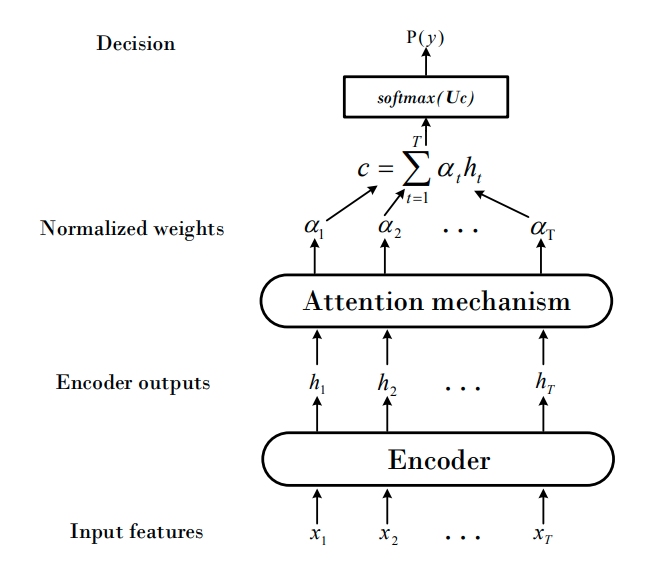
\includegraphics[width=0.5\textwidth]{figures/attention_arch.png}
                \caption{Attention-based end-to-end model for KWS.}
                \label{fig:attention_arch}
            \end{center}
        \end{figure}

        \begin{description}
            \item[Feature Extraction] The positive training sample has a frame length of $T = 1.9$ seconds which ensures the entire wake-up word is included. 
            Accordingly, in the attention models, the input window has set to 189 frames to cover the length of the wake-up word.
            Each audio frame was computed based on a 40-channel Mel-filterbank with 25ms windowing and 10ms frame shift. 
            Then the filterbank feature was converted to per-channel energy normalized (PCEN) [21] Mel-spectrograms.

            \item[Deep Neural Network] The overall architecture can be seen in figure \ref{fig:attention_arch}.
            The end-to-end system consists of an encoder and an attention mechanism. 
            The encoder transforms the input features into a high level representation using simple RNNs. 
            Then the attention mechanism weights the encoder features and generates a fixed-length vector.
            Two types of attention were investigated, average attention and soft attention
            \begin{itemize}
                \item \textbf{Average attention}: The \textit{Attention} model does not have trainable parameters and the $\alpha_{t}$ is set as the average of $T$:
                \begin{equation}
                    \alpha_{t} = \frac{1}{T}
                \end{equation}

                \item \textbf{Soft attention}: This attention method is borrowed from speaker verification \cite{abc}, the model learns the shared-parameter non-linear attention weights.
                First, model learns a scalar score $e_{t}$:
                \begin{equation}
                    e_{t} = v^{T}\tanh(Wh_{t} + b)
                \end{equation}

                Then the normalized weight $\alpha_{t}$ are computed using these scalar scores:
                \begin{equation}
                    \alpha_{t} = \frac{\exp(e_{t})}{\sum_{j=1}^{T}{\exp(e_{j})}}
                \end{equation}

            \end{itemize}

            Finally, by linear transformation and softmax function, the vector becomes a score used for keyword detection.
            To improve end-to-end approach, further encoder architectures were explored, including LSTM, GRU and CRNN.

            \item[Posterior Handling] Unlike some other approaches, the end-to-end system outputs a confidence score directly without post-processing.
            The attention-based system is triggered directly when the $p(y=1)$ exceeds a preset threshold.
        \end{description}

        Experiments on real-world wake-up data show that, with similar size of parameters, the attention models outperform Deep KWS by a large margin. 
        With encoder architecture, GRU is preferred over LSTM and the best performance is achieved by CRNN.

    \section{WaveNet-based small-footprint KWS} \label{sec:related_wavenet}

        Article \cite{wavenet} presented a end-to-end stateless temporal modeling which can take advantage of a large context while limiting computation and avoiding saturation issues.
        An architecture was explored based on a stack of dilated convolution layers, effectively operating on a broader scale than with standard convolutions while limiting model size. 
        Further improvement solution was to use with gated activations and residual skip-connections, inspired by the WaveNet style architecture explored previously for text-to-speech applications \cite{wavenet} and voice activity detection \cite{wavenet}, but never applied to KWS at the time the article was published.
        Moreover, ResNets differ from WaveNet models in that they do not leverage skip-connections and gating, and apply convolution kernels in the frequency domain, drastically increasing the computational cost.
        In addition, the long-term dependency the model can capture is exploited by implementing a custom ``end-of-keyword'' target labeling, increasing the accuracy of the model.

        \begin{description}

            \item[Feature Extraction] The acoustic features are 20-dimensional log-Mel filterbank energies (LFBEs), extracted from the input audio every 10ms over a window of 25ms.
            
            \item[Deep Neural Network] WaveNet was initially proposed in \cite{wavenet}, as a generative model for speech synthesis and other audio generation tasks.
            It consists in stacked causal convolution layers wrapped in a residual block with gated activation units as depicted in figure \ref{fig:wavenet_arch}.

            \begin{itemize}
                \item \textbf{Dilated convolution}: Standard convolutional networks cannot capture long temporal patterns with reasonably small models due to the increase in computational cost yielded by larger receptive fields. 
                Dilated convolutions skip some input values so that the convolution kernel is applied over a larger area than its own.
                The network therefore operates on a larger scale, without the downside of increasing the number of parameters. 
                The receptive field $r$ of a network made of stacked convolutions indeed reads:
                \begin{equation}
                    r = \sum_{i}{d_{i}(s_{i}-1)}
                \end{equation}

                where $d_i$ refers to the dilation rate ($d_i = 1$ for normal convolutions) and $s_i$ the filter size of the i-th layer. 

                \item \textbf{Gated activations and residual connections}: Gated activations units - a combination of $tanh$ and $sigmoid$ activations controlling the propagation of information to the next layer - prove to efficiently model audio signals.
                Residual learning strategies such as skip connections are also introduced to speed up convergence and address the issue of vanishing gradients posed by the training of models of higher depth. 
                Each layer yields two outputs: one is directly fed to the next layer as usual, but the second one skips it. 
                All skip-connections outputs are then summed into the final output of the network. 
                A large temporal dependency, can therefore be achieved by stacking multiple dilated convolution layers.
            \end{itemize}

            \begin{figure}
                \begin{center}
                    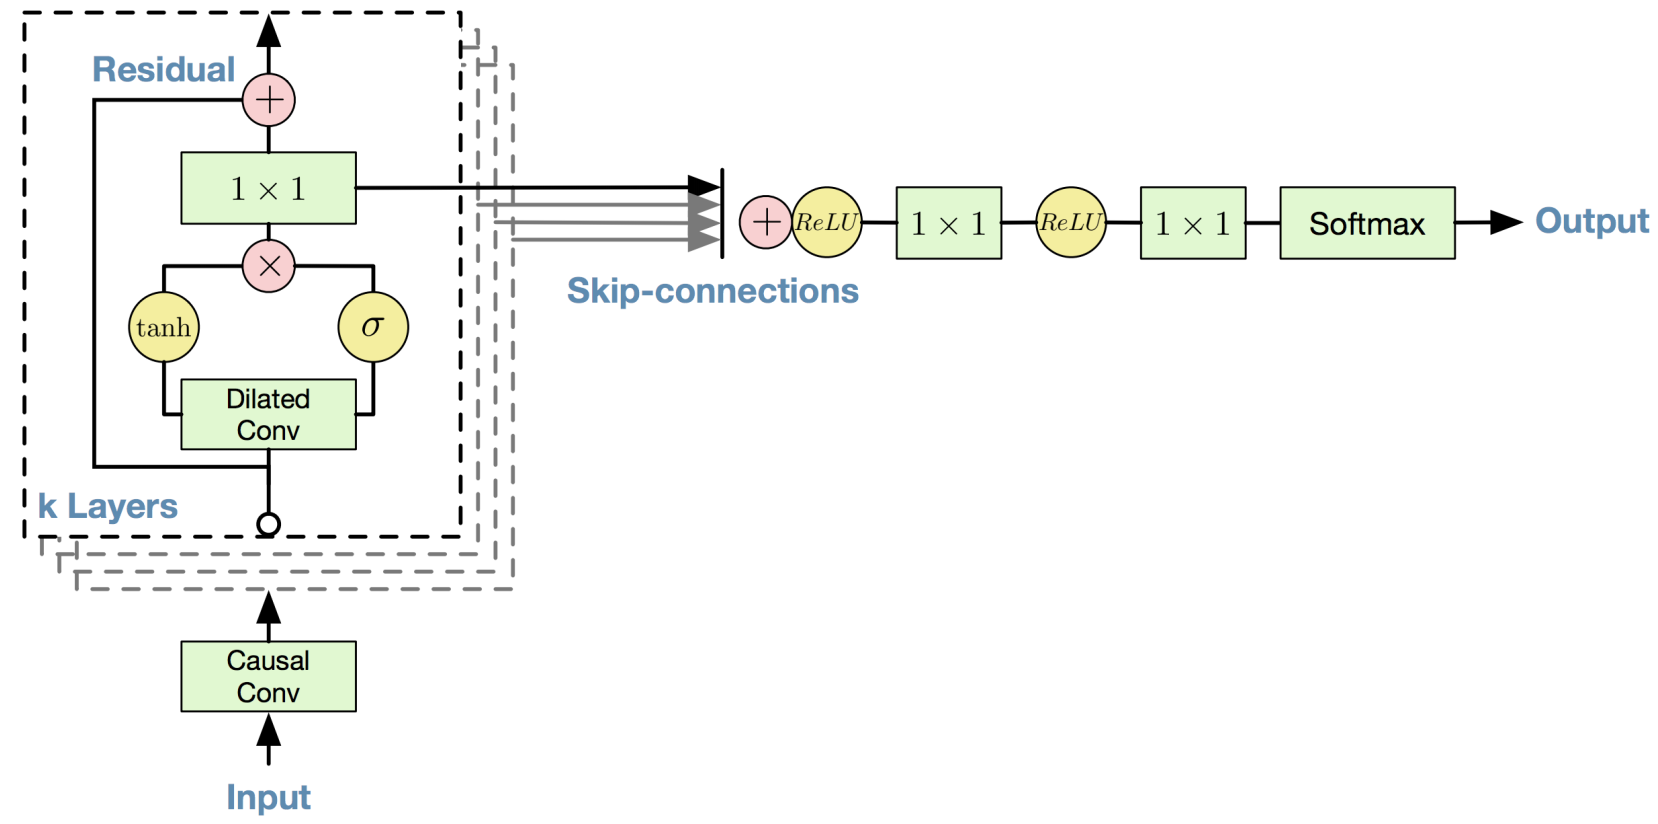
\includegraphics[width=0.7\textwidth]{figures/wavenet_arch.png}
                    \caption{WaveNet architecture.}
                    \label{fig:wavenet_arch}
                \end{center}
            \end{figure}

            \item[Posterior Handling] Like Deep KWS approaches, the end-to-end system computes smoothed posteriors by averaging the output of a sliding context window containing $w_{smooth}$ frames. However, the models do not require any postprocessing step besides smoothing, as opposed to others multi-class models.
            Indeed, the system triggers when the smoothed keyword posterior exceeds a pre-defined threshold.
        \end{description}



    % !TEX root = ../main.tex
\chapter{Proposed Model} \label{chap:proposed_model}
    \section{Introduction}\label{sec:proposed_intro}

    \section{Proposed Architecture}\label{sec:proposed_arch}
    	\subsection{End-to-end Architecture}
    	\subsection{Deformable Convolutional Network}
    	\subsection{Attention Mechanism}

    \section{Experimental Setup}\label{sec:proposed_setup}
    	\subsection{Dataset}
    	\subsection{Data Augmentation}
    	\subsection{Configurations}


    \section{Results}
    	\subsection{Baselines}
    	\subsection{Proposed Model}
    	\subsection{Discussion}
    	


    \cleardoublepage
    \footnotesize
    \ihead[]{Bibliography}
    \bibliography{main}
    \normalsize

\end{document}
